\clearpage
\section{Arduino Quantum Receiver}

\begin{refsection}

\begin{tcolorbox}	
\begin{tabular}{p{2.75cm} p{0.2cm} p{10.5cm}} 	
\textbf{Student Name}  &:&  Eduardo Fernandes (2019/06/15 - 2019/09/14)\\
\textbf{Goal}          &:& Implement the QKD reception module in an Arduino (Coincidence Detector, QBER, Source and Sink blocks).\\
\textbf{Directory}              &:& sdf/arduino\_quantum\_rx
\end{tabular}
\end{tcolorbox}


\subsection{Simulation Analysis - QKD reception module}

\begin{figure}[H]
	\centering
	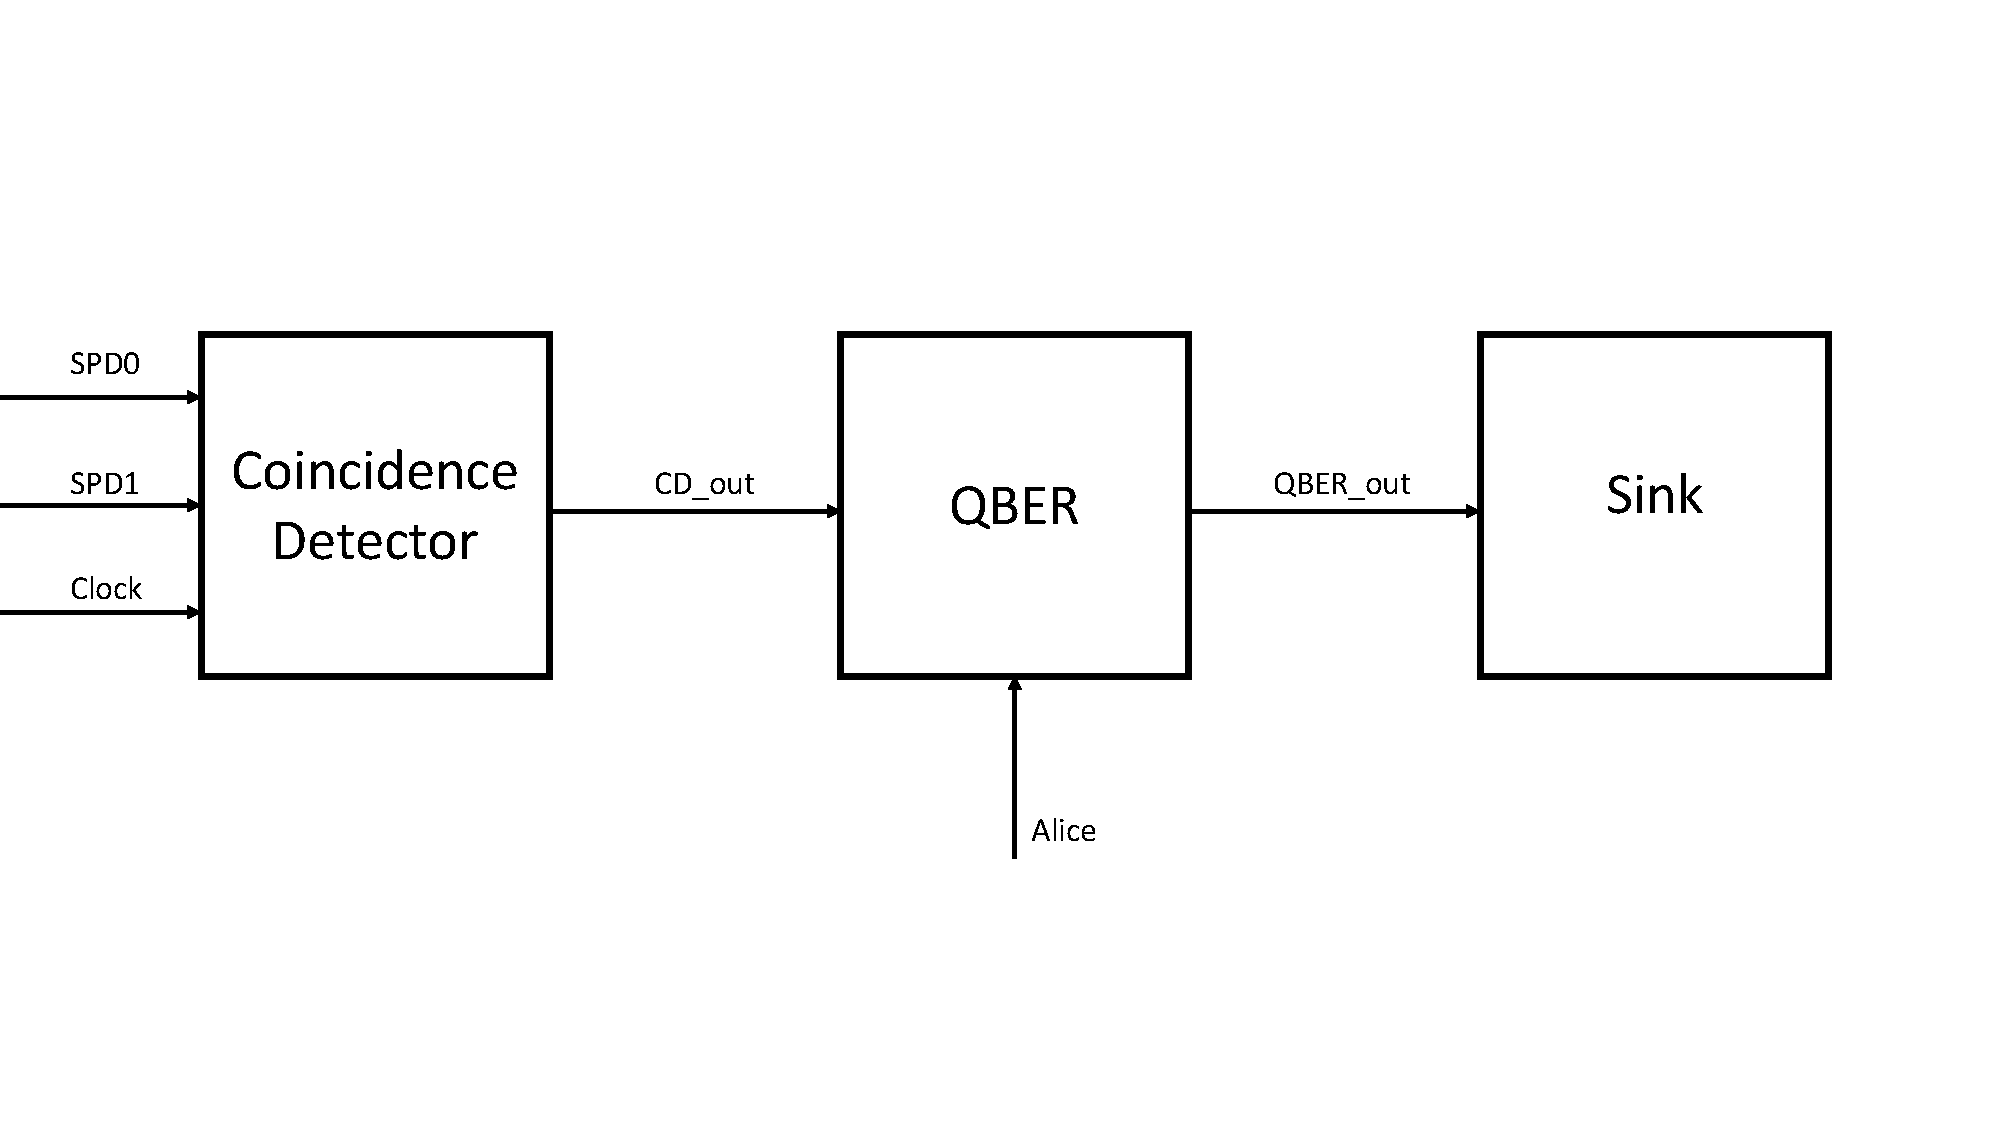
\includegraphics[width=1\linewidth]{./sdf/arduino_quantum_rx/figures/generalDiagram.pdf}
	\caption{General block diagram of QKD a quantum receiver module.}
	\label{fig:arduino}
\end{figure}

This system emulates the QKD reception module of a quantum communication system. It is comprised by three main blocks. The first is the coincidence detector  which contains three inputs: the signals provenient from the single-photon detectors 0 and 1 and a clock signal used to keep all blocks synchronized, as it provides the sampling frequency. In addition, this block outputs a signal containing a state corresponding to the input values. That signal will be the input of the next block, the QBER, this block compares two input binary signals, one provenient from the coincidence detector and one other coming directly from Alice's side, and outputs a binary signal with a zero if both input bits are equal and a one if they differ. Additionally, this block does statistical analysis on the QBER and outputs a file with the results of this analysis. Finally, the output signal of the QBER block enters a Sink block, not generating any output. 

\subsection{Emulation in NetXPTO Simulator}

\vspace{11pt}

\begin{figure}[H]
	\centering
	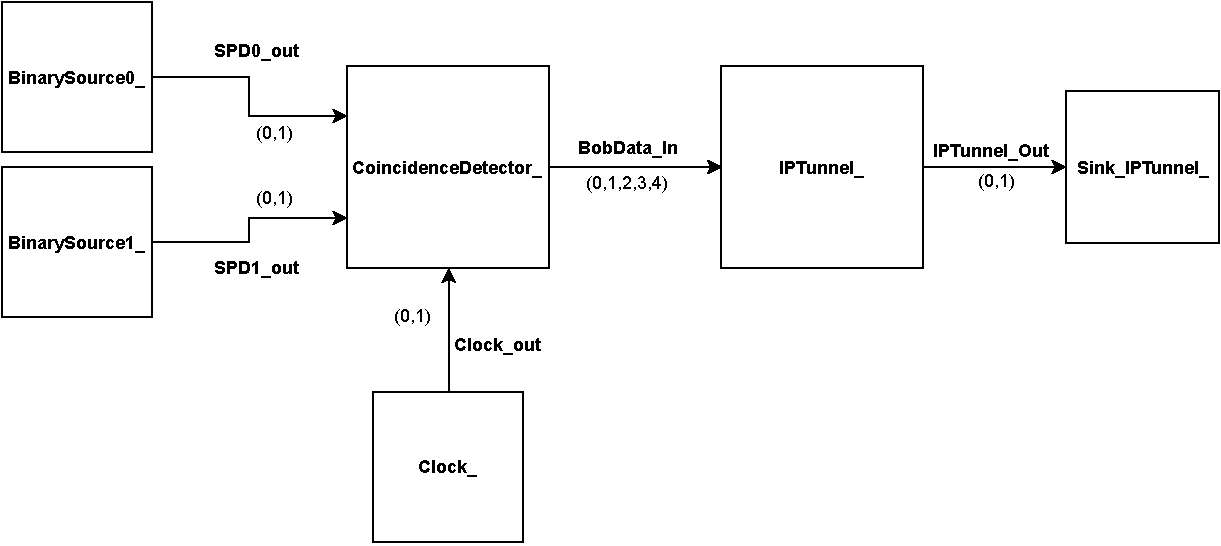
\includegraphics[width=0.9\linewidth]{./sdf/arduino_quantum_rx/figures/NetXPTO_implementation.pdf}
	\caption{Block diagram of a quantum receiver system emulated in NetXPTO.}
	\label{fig:netxpto}
\end{figure}

Here are presented and described the implementation of the 6 modules needed. The first two are the BinarySource0\_ and the BinarySource1\_ which emulate the received signals provenient from the single-photon detectors 0 and 1, respectively. These signals are the inputs of the CoincidenceDetector\_ block, which in its turn, outputs a real signal that has five possible values: 5 if it is a control qubit (which should be discarded by the upper layer), 3 if no-click has been detected, 2 if both detectors clicked, 1 if bit one was measured, and finally, 0 if bit zero was measured. Next, we have the BinarySource2\_ block which has a binary output signal representing the measured value that arrives from the quantum channel from Alice side. Another existent block is the QBER\_ which is responsible for some of the post processing tasks, more specifically, the QBER estimation and outputs a real signal with the quantum channel QBER. Finally there is the Sink\_QBER\_ blocks, which, accpets one binary input signal provenient from the QBER\_ block and does not produce any output signals, it simply takes samples out of the circular buffer until it is empty.\\ \\

The following input parameters were defined for the blocks listed in figure \ref{fig:netxpto}:

\begin{itemize}
	\item BinarySource0\_:
	\begin{itemize}
		\item setMode(BinarySourceMode::DeterministicCyclic)
		\item setBitPeriod(1e-11)
		\item setBitStream("1")
		\item setNumberOfBits(10000);
	\end{itemize}
	\clearpage
	\item BinarySource1\_:
	\begin{itemize}
		\item setMode(BinarySourceMode::DeterministicCyclic)
		\item setBitPeriod(1e-11)
		\item setBitStream("0")
		\item setNumberOfBits(10000);
	\end{itemize}
	
	\item BinarySource2\_:
	\begin{itemize}
		\item setMode(BinarySourceMode::DeterministicCyclic)
		\item setBitPeriod(1e-11)
		\item setBitStream("1")
		\item setNumberOfBits(10000);
	\end{itemize}
	
	\item CoincidenceDetector\_;
	
	\item QBER\_;
	
	\item QBER\_Sink\_.
\end{itemize}





\subsection{Simulation Analysis - Arduino Implementation}

In order to utilize the same project running over NetXPTO simulator using Arduino some changes in the source code had to be made once this technology uses C/C++ language features while relying on special rules of code structuring.

The outputs to the console have to be made through the arduino serial monitor using the function Serial.print() instead of making use of cout, cin or cerr; 

The implementation of a non-specialized template methods must be visible to a translation unit that uses it. The compiler must be able to see the implementation in order to generate code for all specializations in your code. This can be achieved in two ways: either by moving the implementation, the cpp file, inside the header or if you want to keep it separate, move it into a different header which you include in your original header.

Arduino does not recognize objects of type std::initializer\_list<T>, which are a lightweight proxy object that provides access to an array of objects of type const T, so instead we have to use vector containers in order to initialize the constructors attributes.


\subsection{Arduino Implementation - System Montage}
\begin{figure}[H]
	\centering
	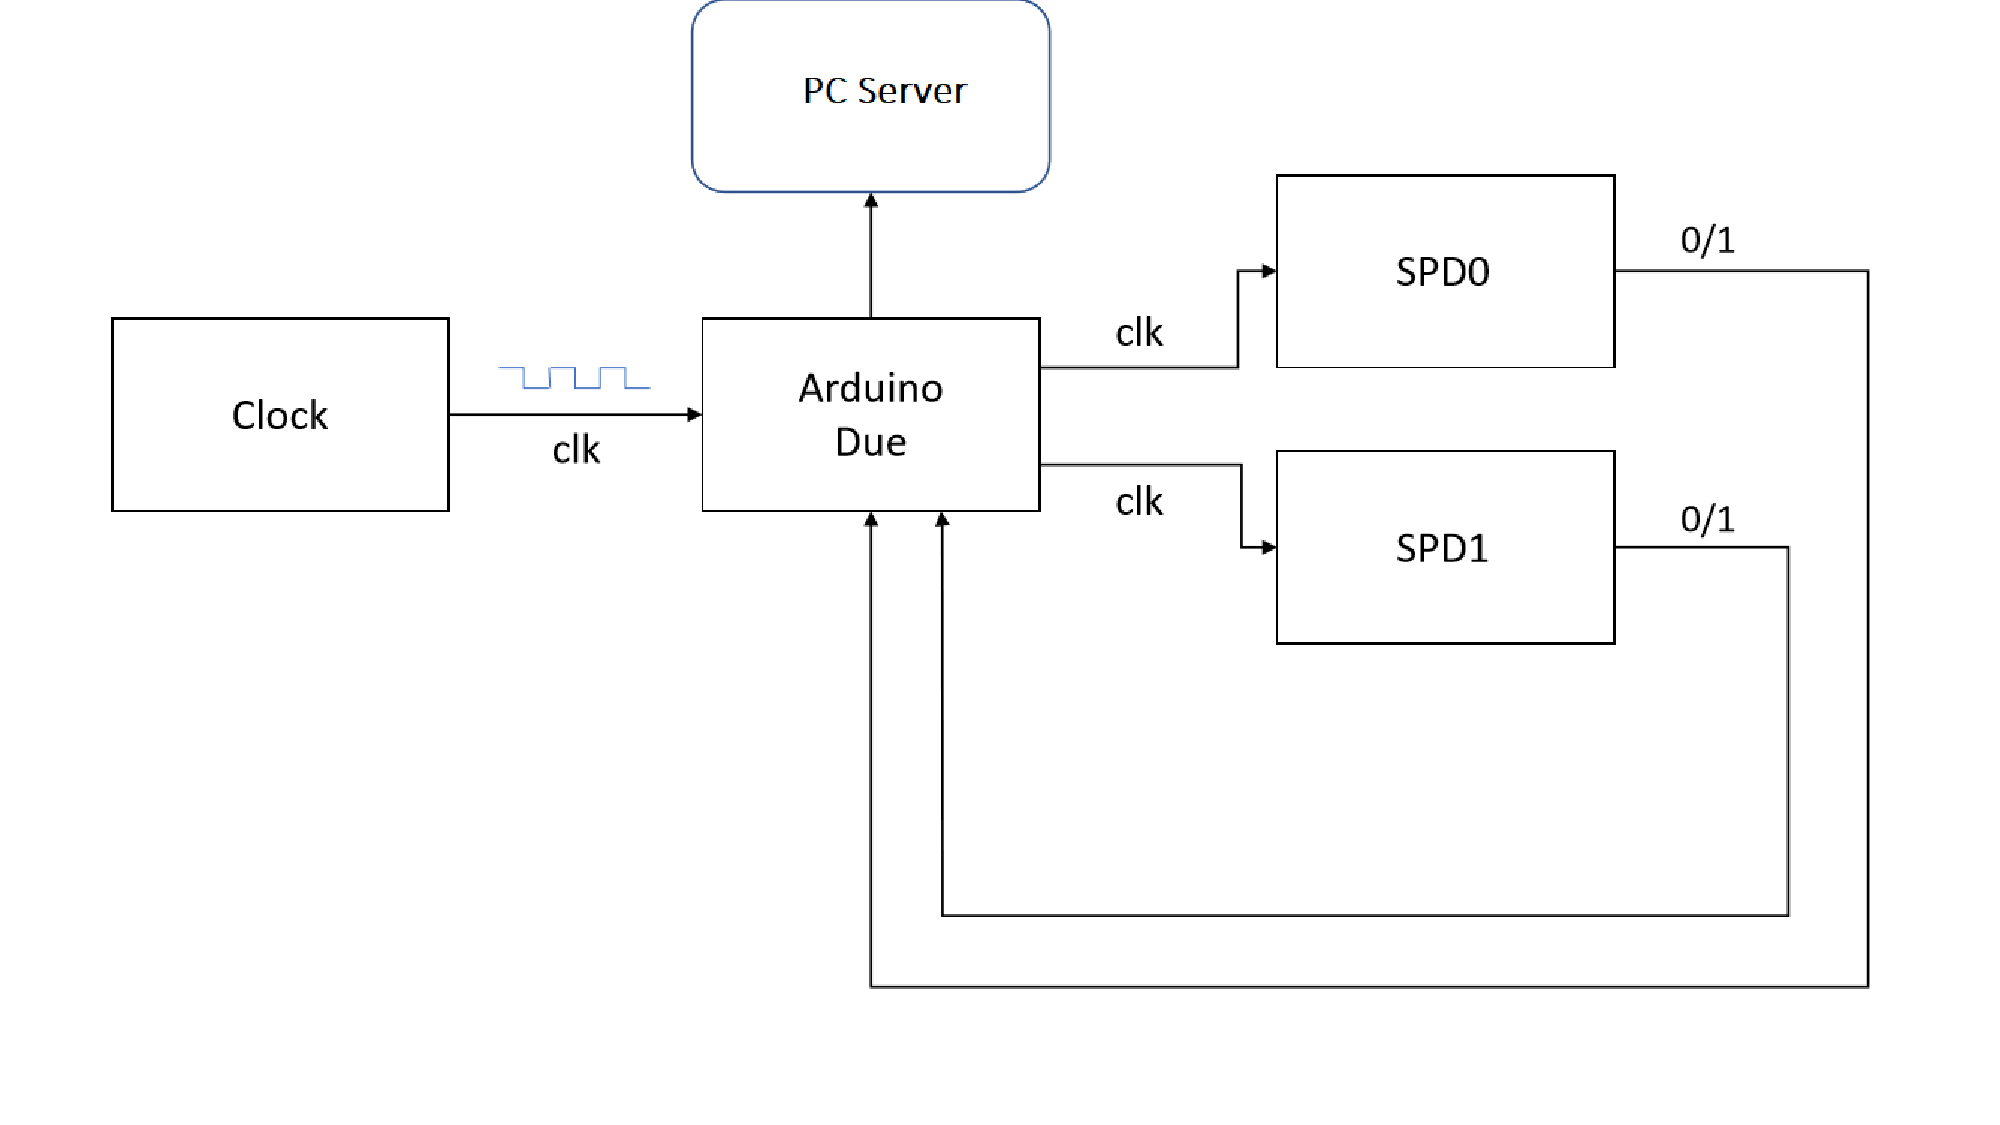
\includegraphics[width=1\linewidth]{./sdf/arduino_quantum_rx/figures/montageDiagram.pdf}
	\caption{Arduino implementation.}
	\label{montage}
\end{figure}



\subsection{Open Issues}

\clearpage
\subsection{Visual Studio 2019 - Installation guide (Current version: 16.2.3)}

\subsubsection{Step 1}

The first thing to do is to download the bootstrapper file of this software through the following link: https://visualstudio.microsoft.com/pt-br/downloads/. As seen below in figure \ref{vstudio} one of three available versions can be choosen.

\begin{figure}[H]
	\centering
	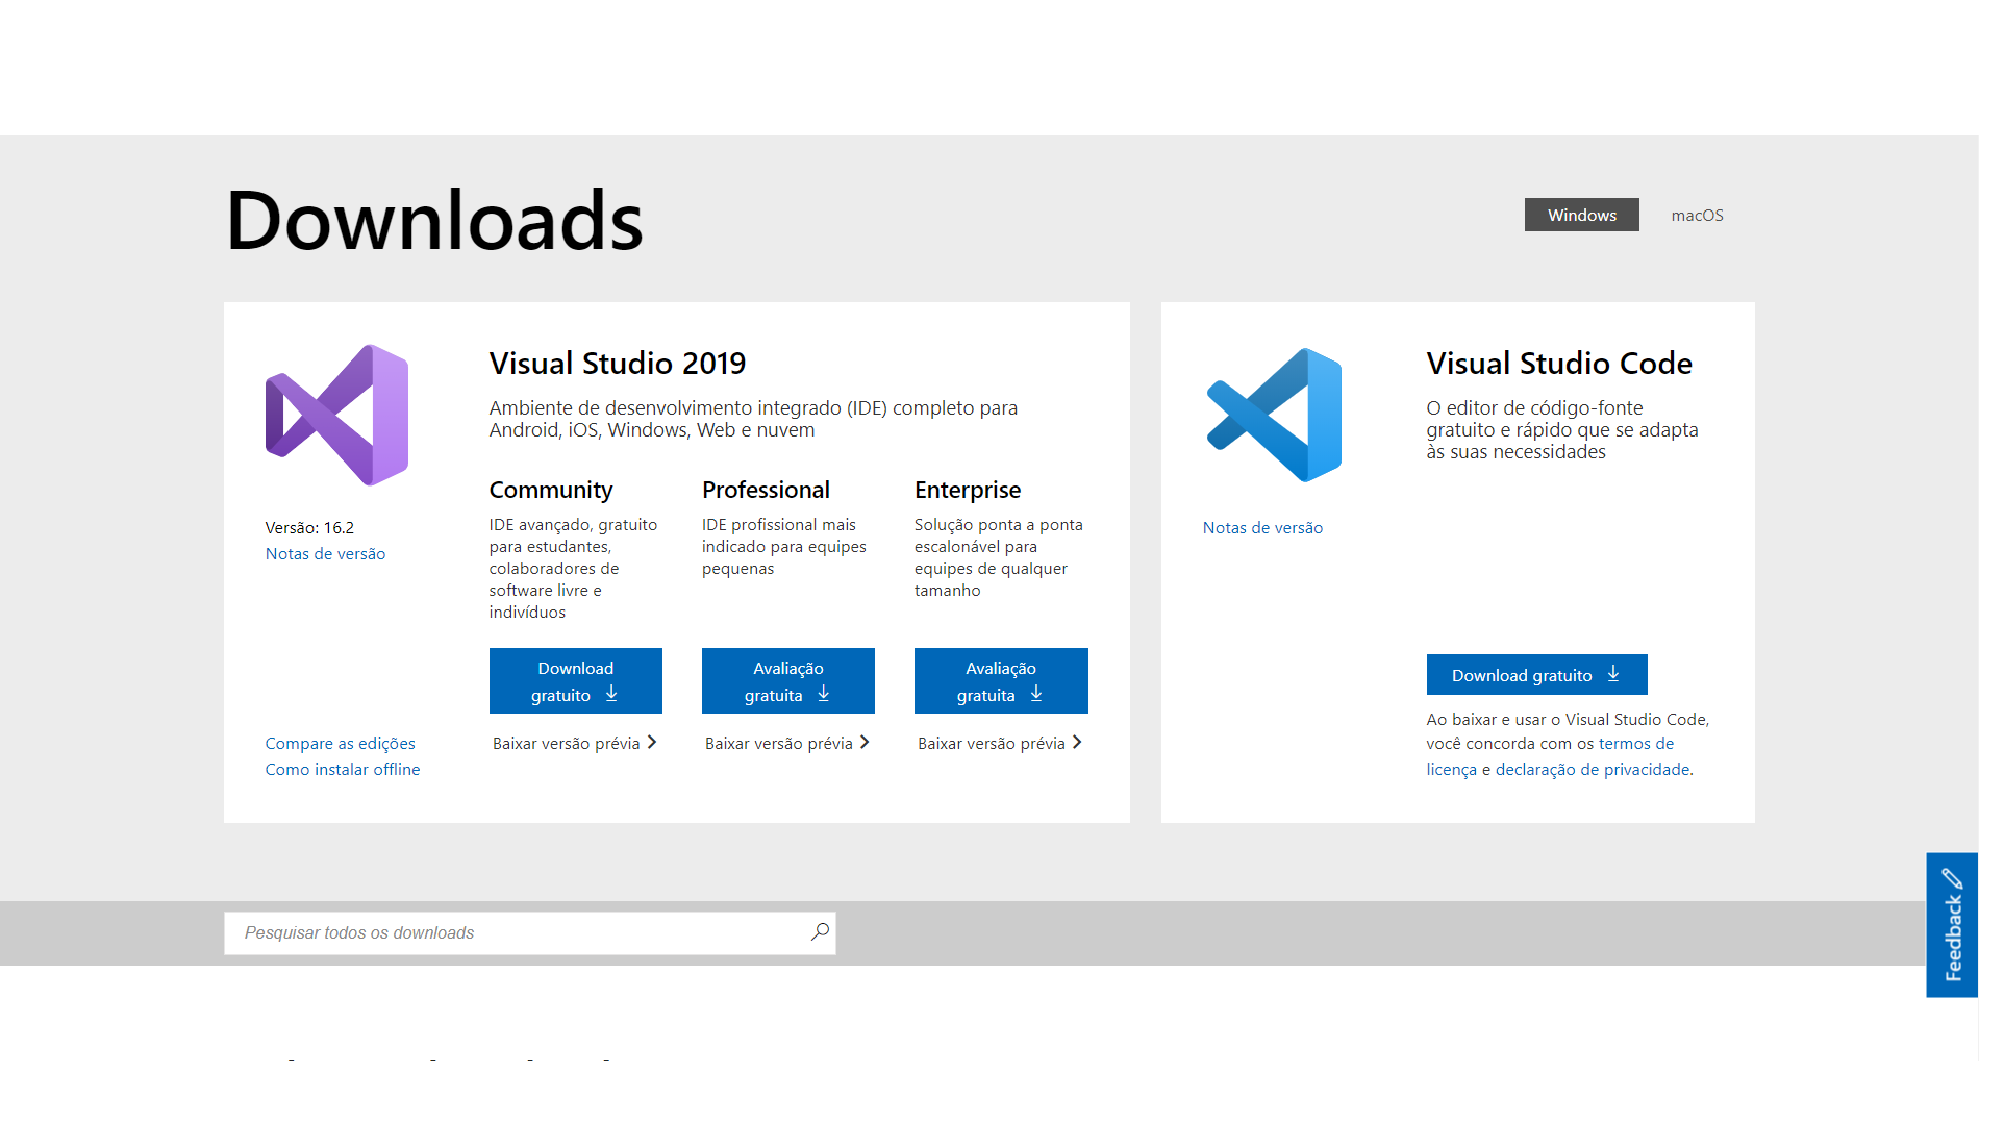
\includegraphics[width=1\linewidth]{./sdf/arduino_quantum_rx/figures/vsDownload.pdf}
	\caption{Download page of Visual Studio IDE software.}
	\label{vstudio}
\end{figure}


\subsubsection{Step 2}

Execute the installer file, which you can use to customize your installation by selecting the feature sets or workloads, individual components, language packs and installation locations, as demonstrated in figure \ref{vstudioWorkloads}. 



\subsubsection{Step 3}

The installation is quite simple and contains few steps for its execution, in case there is any doubt or question you can always get support from https://docs.microsoft.com/en-us/visualstudio/install/install-visual-studio?view=vs-2019.

\begin{figure}[H]
	\centering
	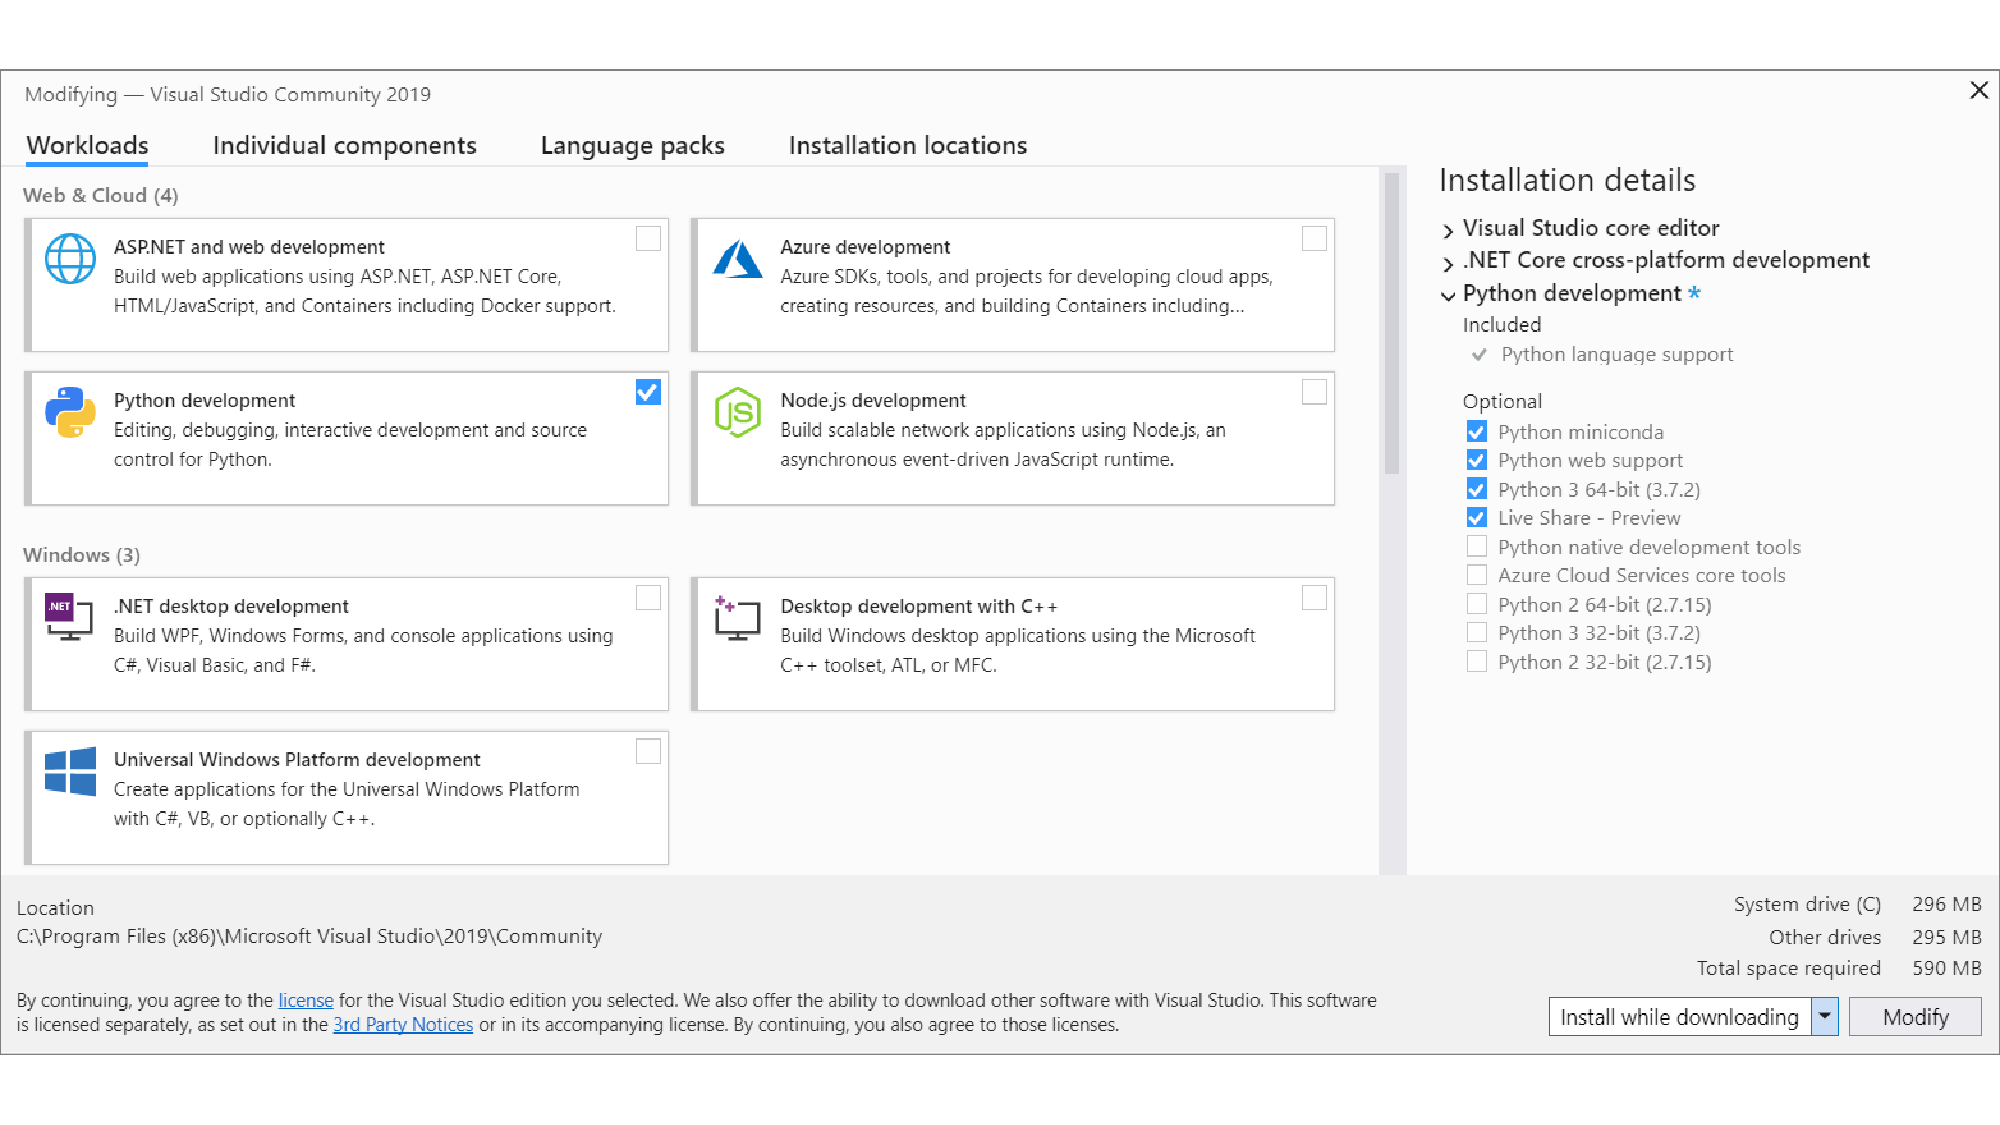
\includegraphics[width=1\linewidth]{./sdf/arduino_quantum_rx/figures/VSworkloads.pdf}
	\caption{Modifying - Visual Studio 2019.}
	\label{vstudioWorkloads}
\end{figure}

\subsection{Arduino IDE - Installation guide (Current version: 1.8.9) for Windows machines}

\subsubsection{Step 1}

Download the latest version of Arduino desktop IDE installer file from https://www.arduino.cc/en/main/software.

\begin{figure}[H]
	\centering
	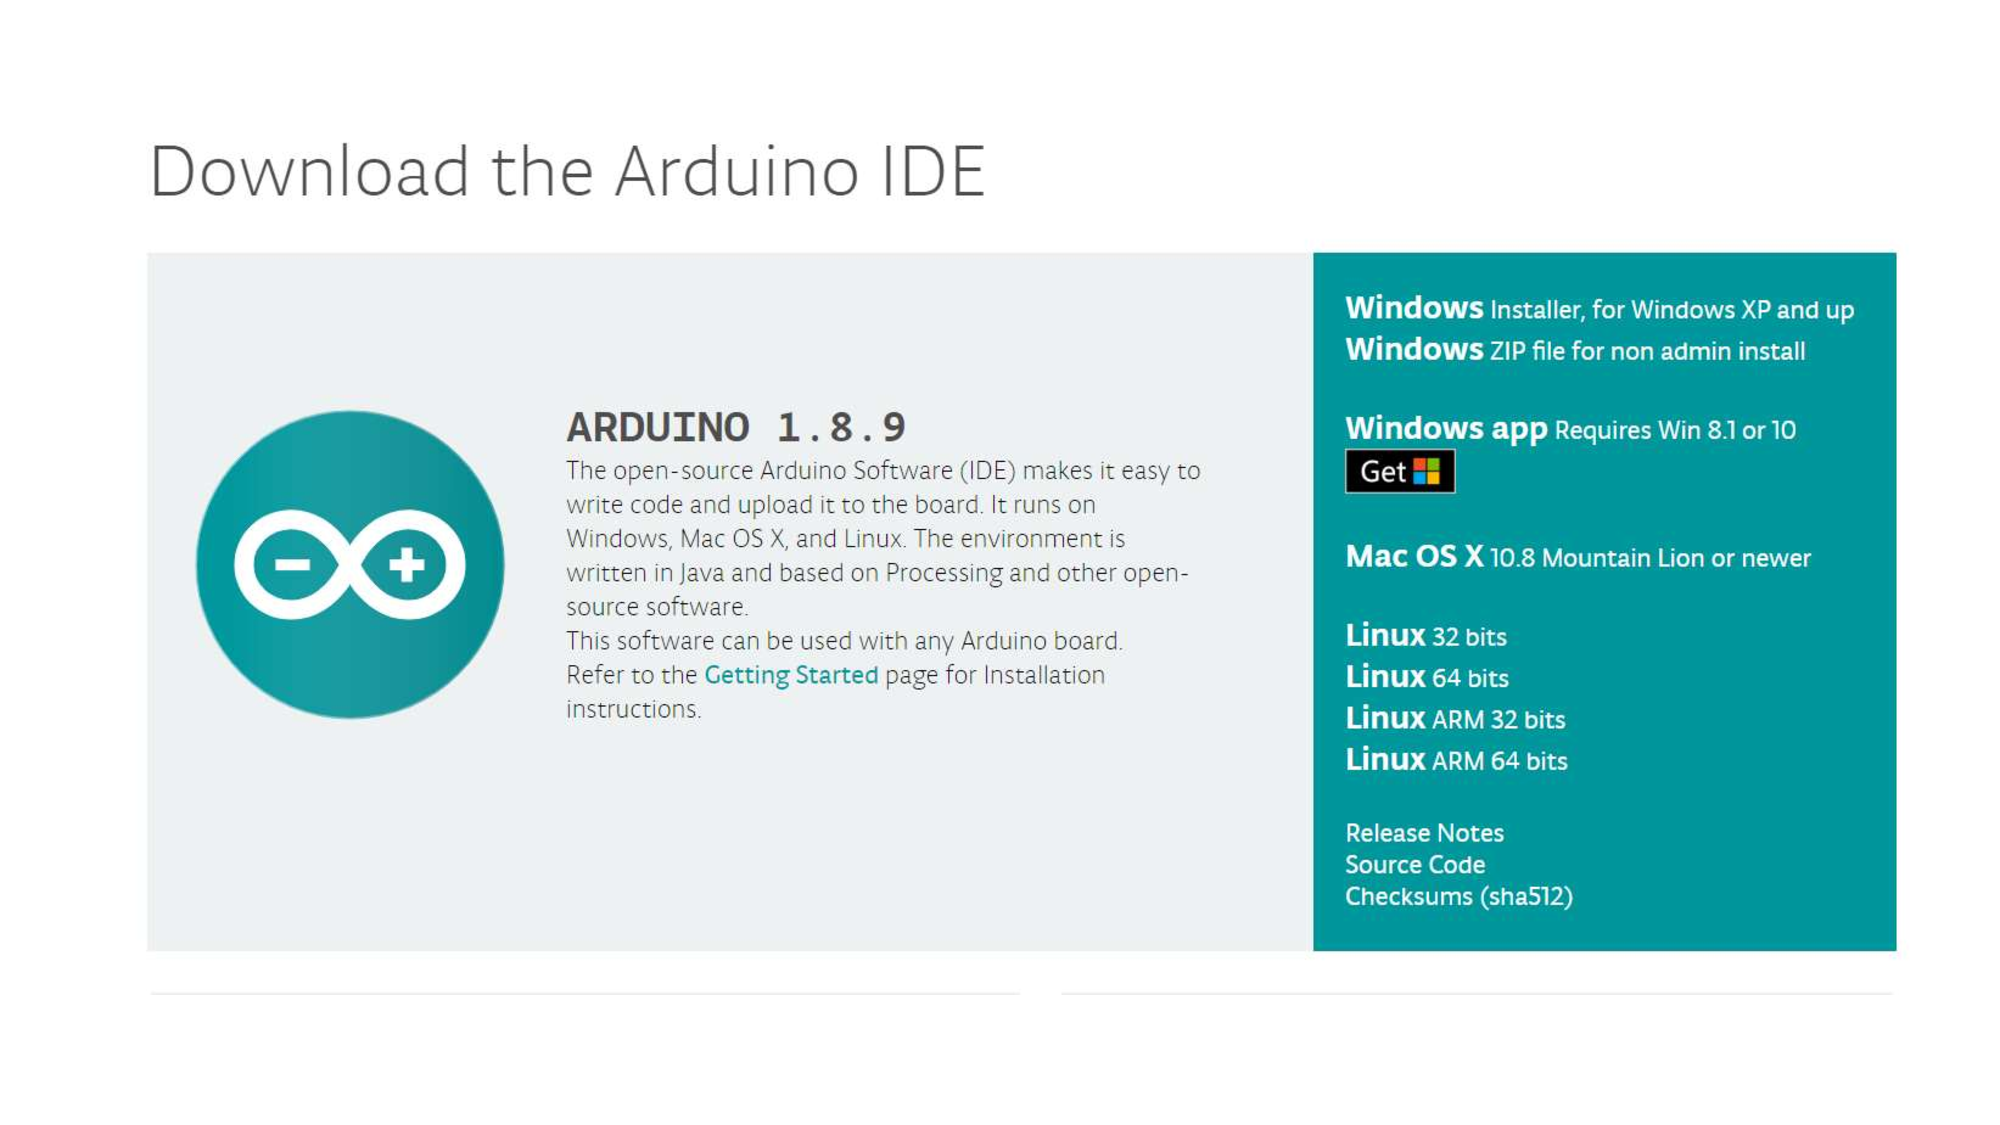
\includegraphics[width=0.86\linewidth]{./sdf/arduino_quantum_rx/figures/arduinoDownload.pdf}
	\caption{Download Arduino IDE software.}
	\label{arduinoDownload}
\end{figure}


\subsubsection{Step 2}

When the download finishes, proceed with the installation and allow the driver installation process when you get a warning from the operating system. Follow the help guide present in https://www.arduino.cc/en/Guide/Windows.

\subsubsection{Step 3}

Proceed with the board specific instructions by going to https://www.arduino.cc/en/Guide/HomePage and selecting the respective board from the list provided, for this specific case we are considering the Arduino Due and so you can use the following link: https://www.arduino.cc/en/Guide/ArduinoDue.

\begin{figure}[H]
	\centering
	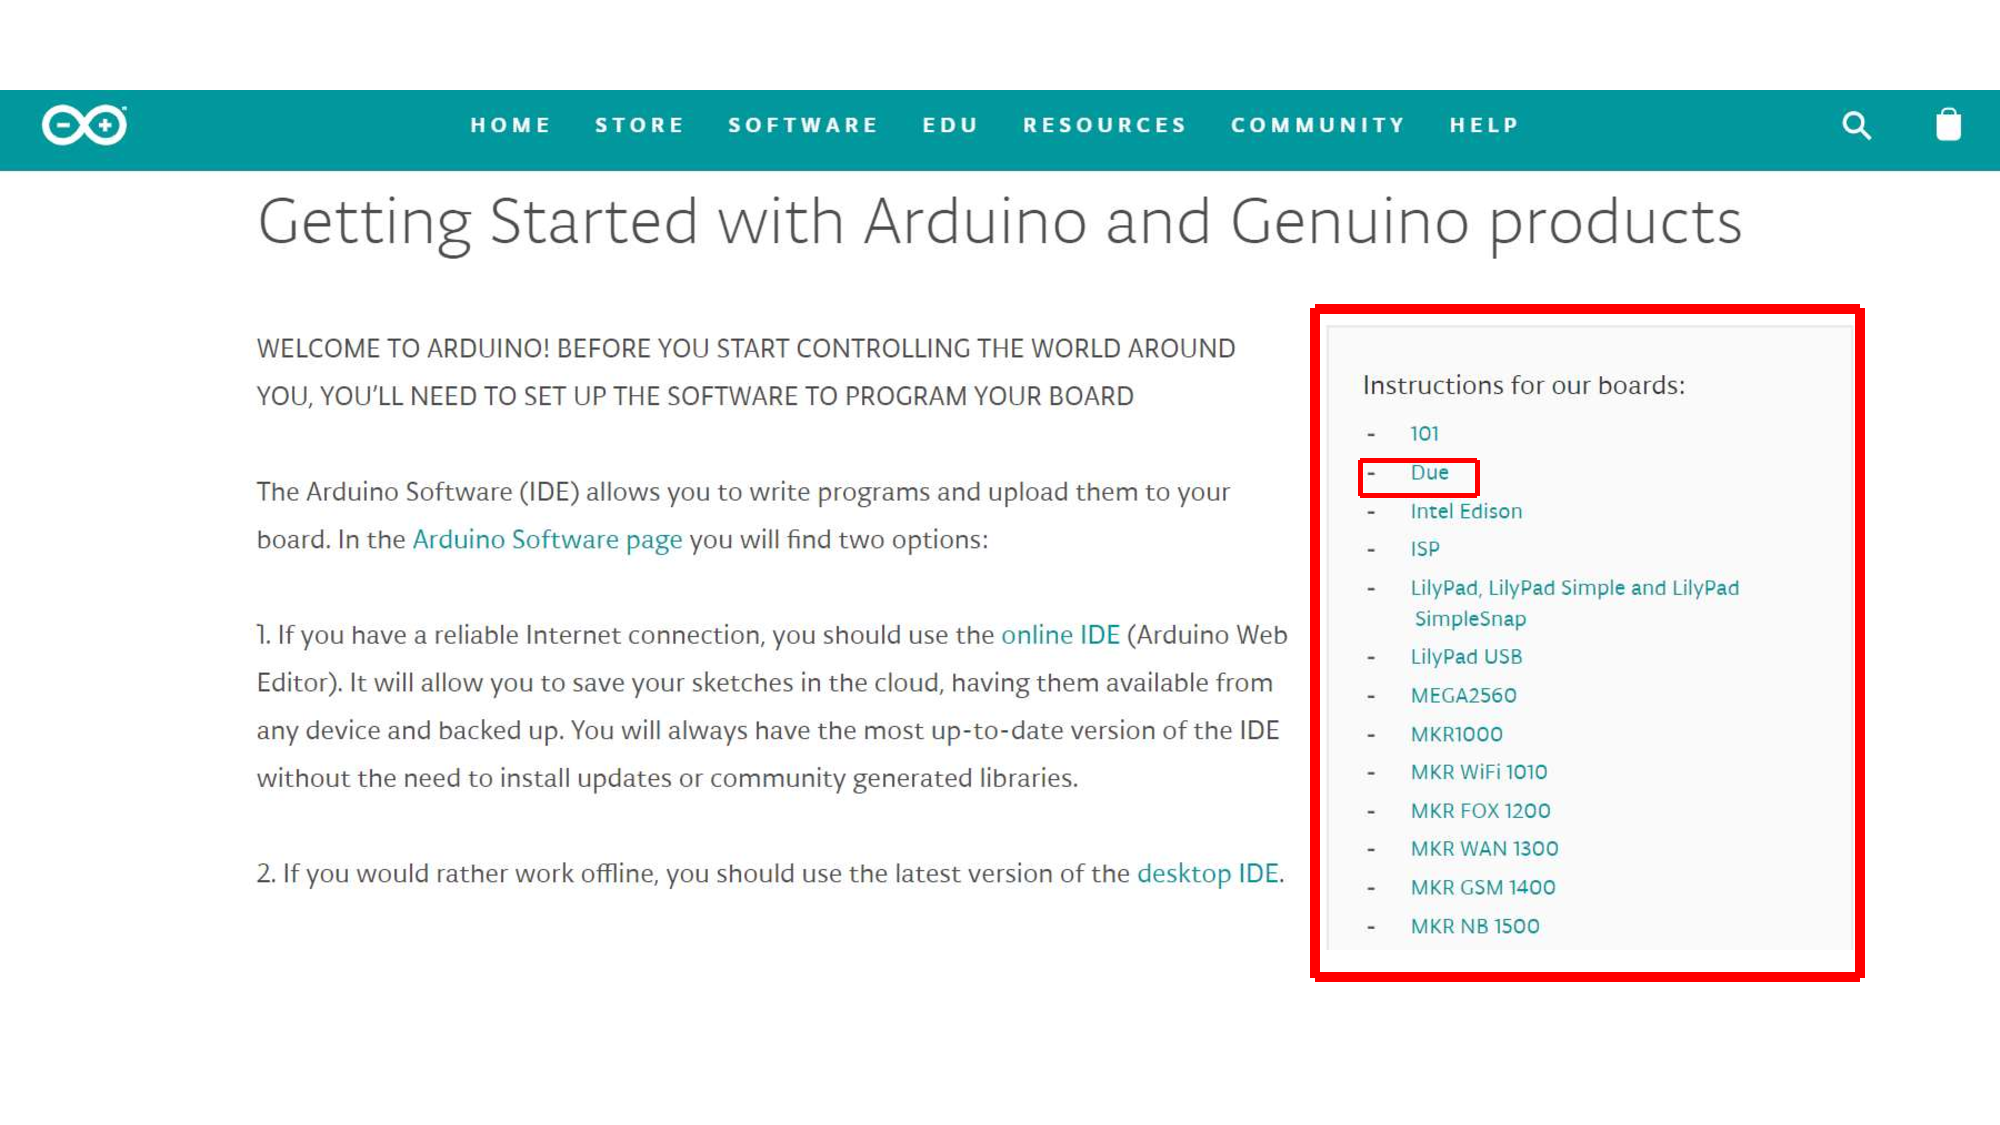
\includegraphics[width=1\linewidth]{./sdf/arduino_quantum_rx/figures/arduinoBoards.pdf}
	\caption{Select instructions for you specific board, in this case, the Arduino Due.}
	\label{arduinoDownload}
\end{figure}

\subsection{Visual Micro - Installation and Setup guide}
Visual Micro is a plugin for Microsoft Visual Studio that helps you creating Arduino compatible cross-platform programs for hundreds of different Arduino compatible micro-controllers. Visual Micro supports projects that contain one or more .ino code files and standard c++ cource code files, just like the Arduino IDE. 


\subsubsection{Step 1}
Download Visual Micro from here https://www.visualmicro.com/page/Arduino-Visual-Studio-Downloads.aspx or it can also be installed and uninstalled from inside the IDE, by opening Visual Studio and clicking "Extensions>Manage Extensions>Online>Arduino IDE for Visual Studio".

\subsubsection{Step 2}
If Visual Studio/Atmel Studio is running, then close it.

\subsubsection{Step 3}
Install Visual Micro by doubleclicking on the "vsix" icon of the downloaded file or in the case you are installing it from within the Visual Studio IDE it will start automatically.

\subsubsection{Step 4}

The first time, after you have installed Arduino for Visual Micro, the Configuration Manager will pop up where you can configure your system. Visual Micro must know the version and installation path of the Arduino IDE software that you have installed in your computer.

\begin{figure}[H]
	\centering
	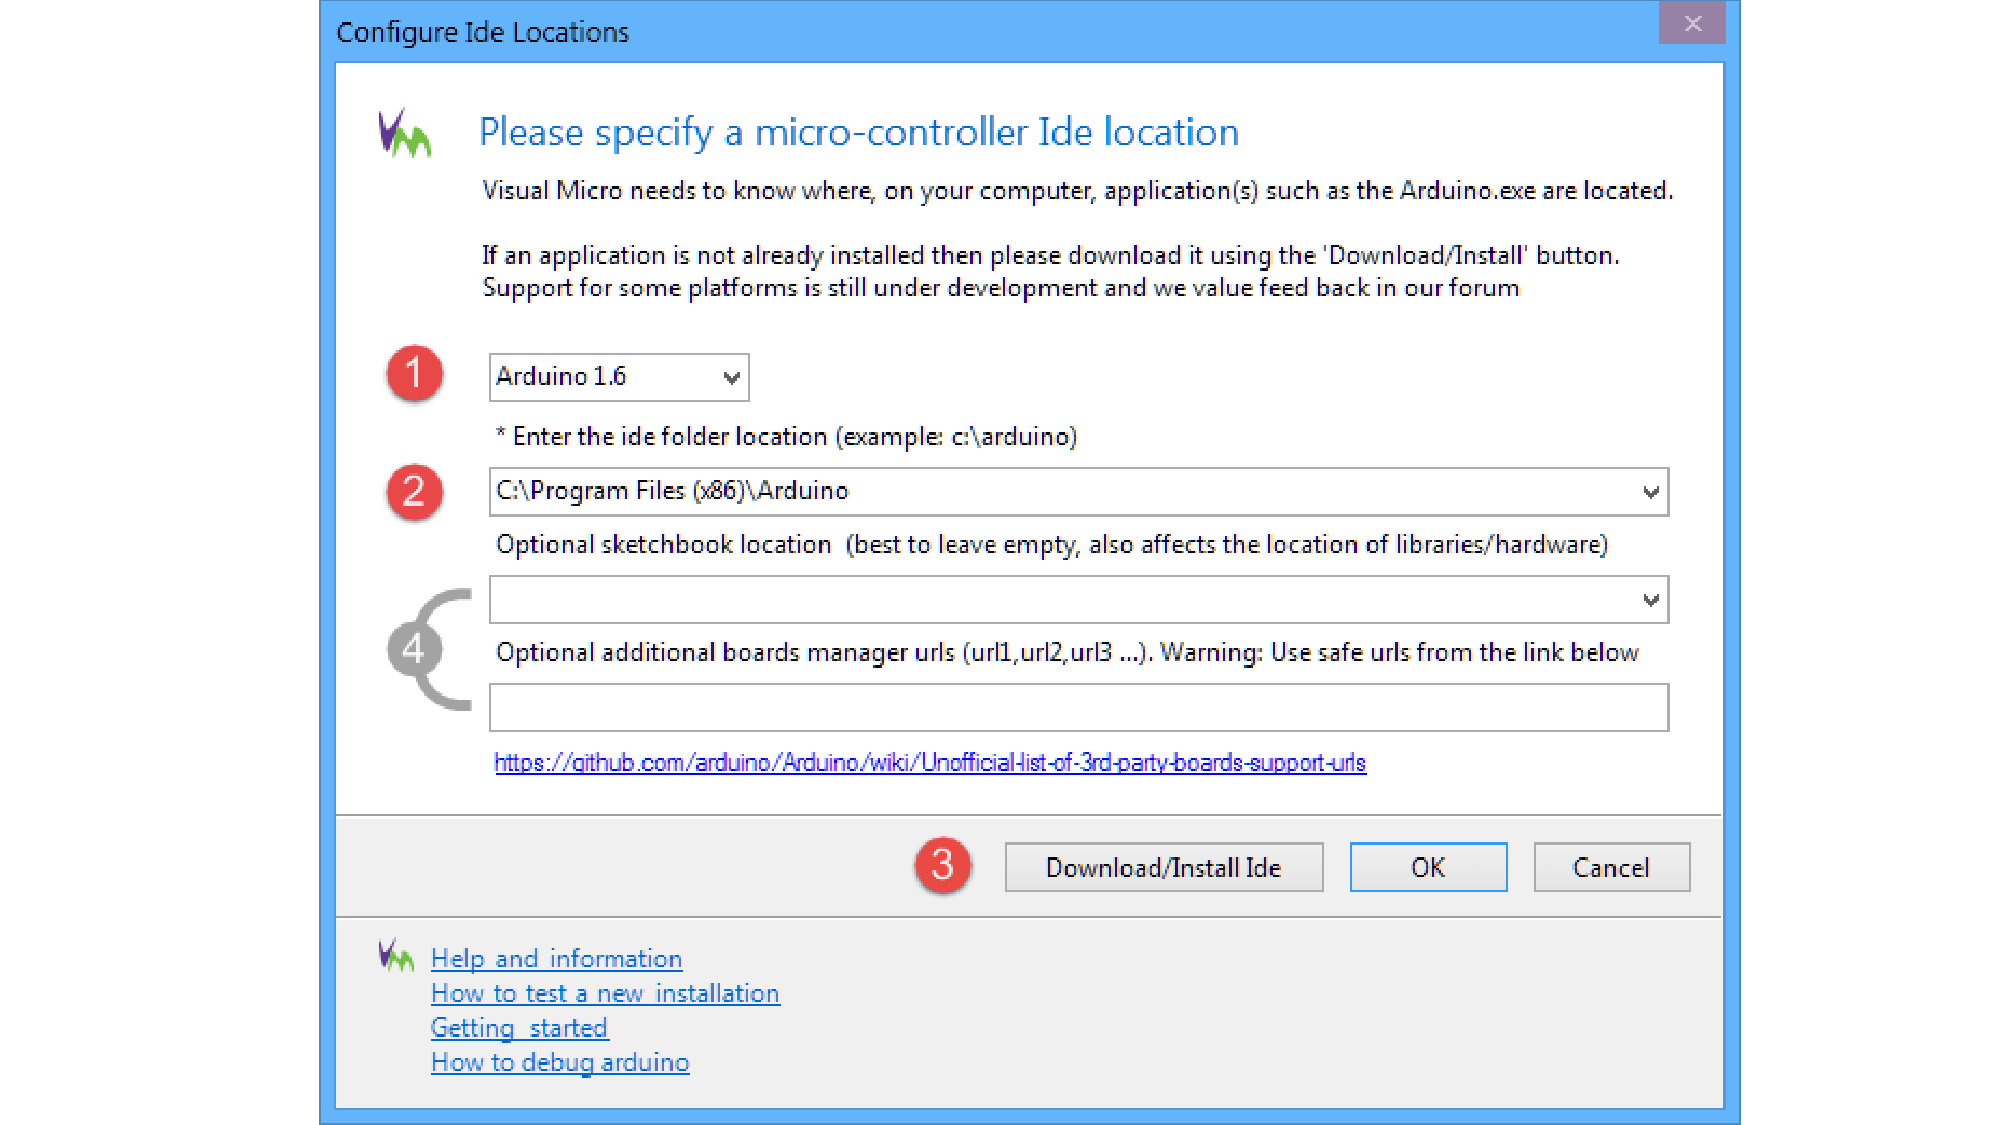
\includegraphics[width=1\linewidth]{./sdf/arduino_quantum_rx/figures/configureIDE.pdf}
	\caption{Configure IDE locations.}
	\label{configureIDE}
\end{figure}

\subsubsection{Step 4}
If you work with different boards that required different IDEs, or if you have multiple versions of the Arduino IDE installed, then repeat the steps above for each IDE. It is possible to switch between configurations with the toolbar presented below in figure \ref{}.

\begin{figure}[H]
	\centering
	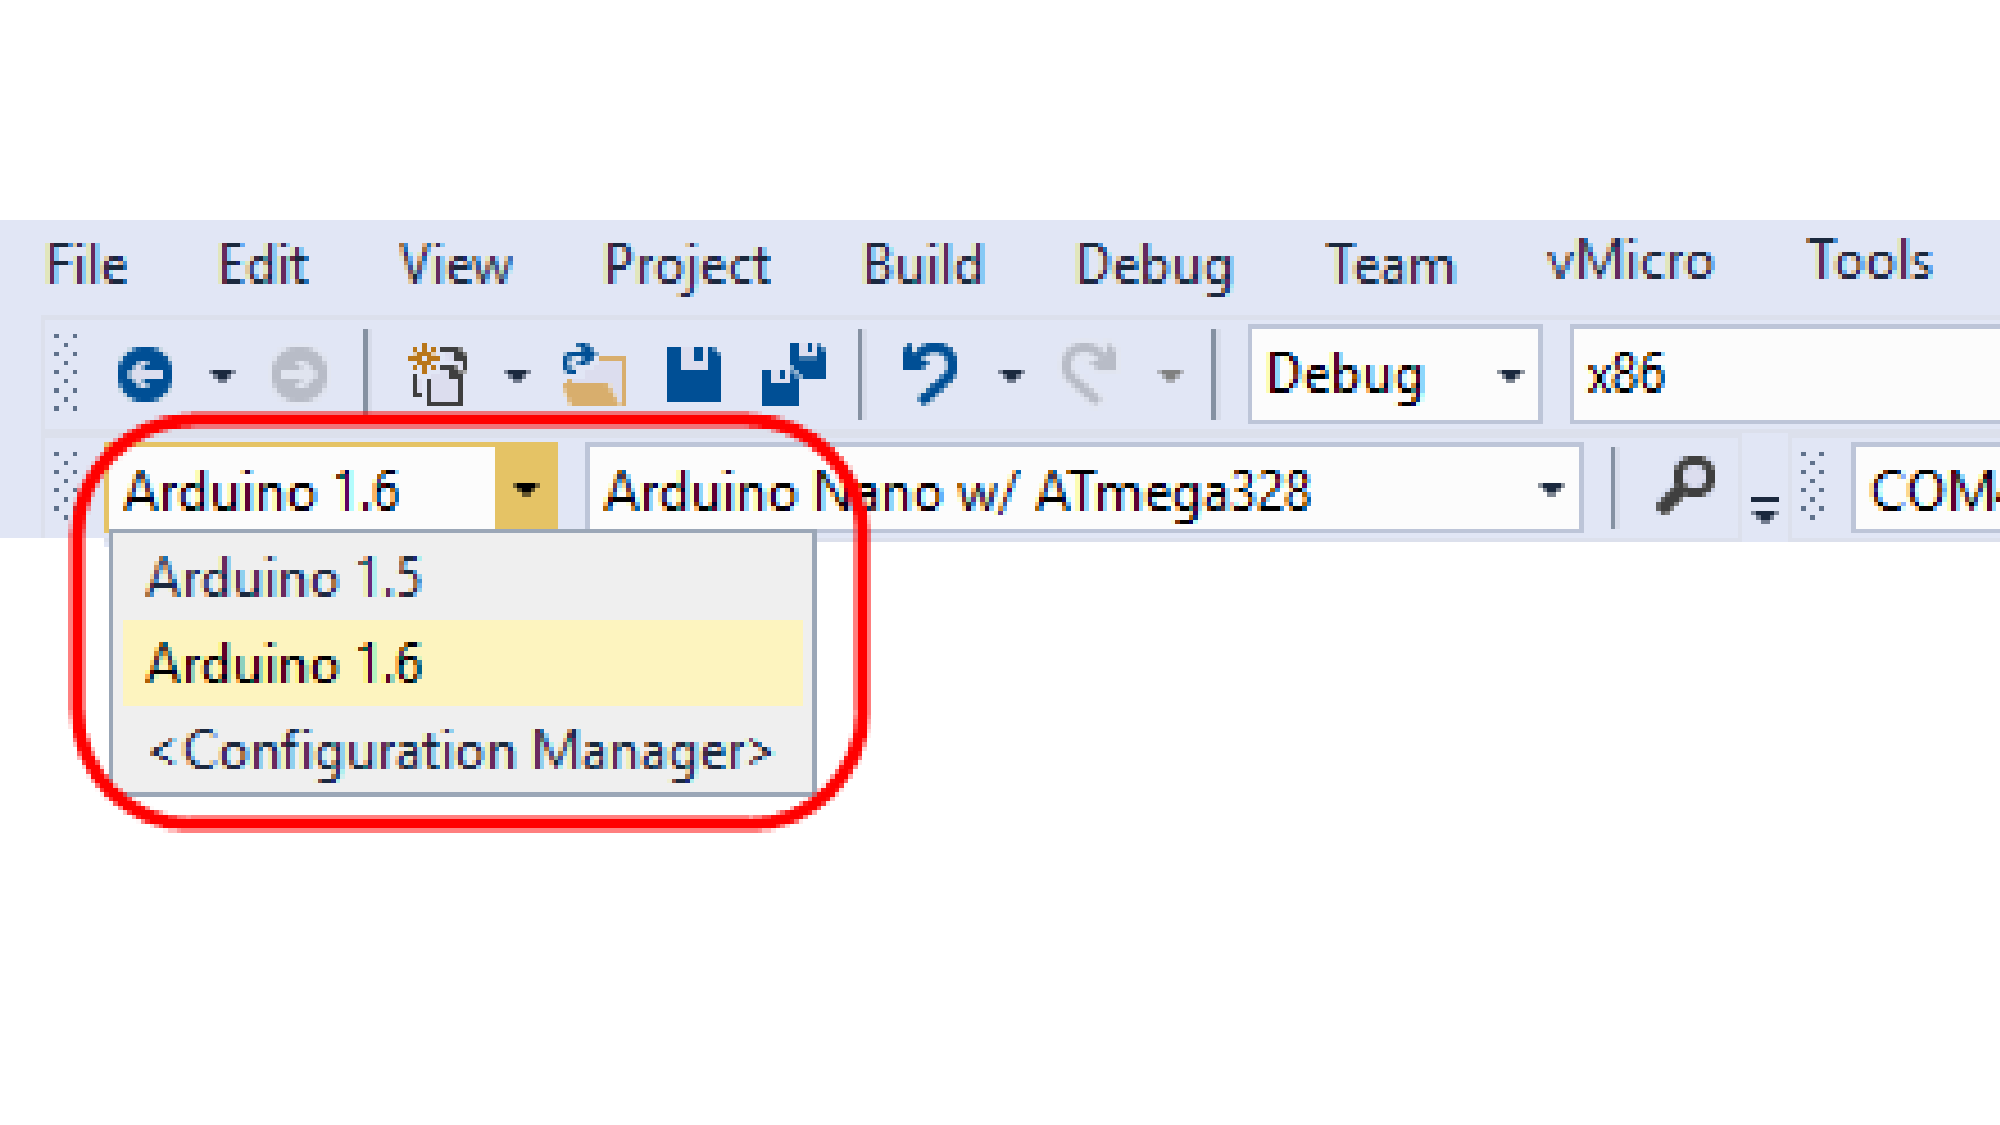
\includegraphics[width=0.7\linewidth]{./sdf/arduino_quantum_rx/figures/multipleIDEversions.pdf}
	\caption{Support for Multiple Versions of the Arduino Softwares.}
	\label{multipleIDEversions}
\end{figure}


\subsubsection{Step 5}

In order to select the board model use the Visual Micro "Micro Boards" toolbar for that purpose, presented below. If the Visual Micro toolbar is missing, then you can show it by right clicking on an empty space in the toolbar area and checking "Micro Boards".


\begin{figure}[H]
	\centering
	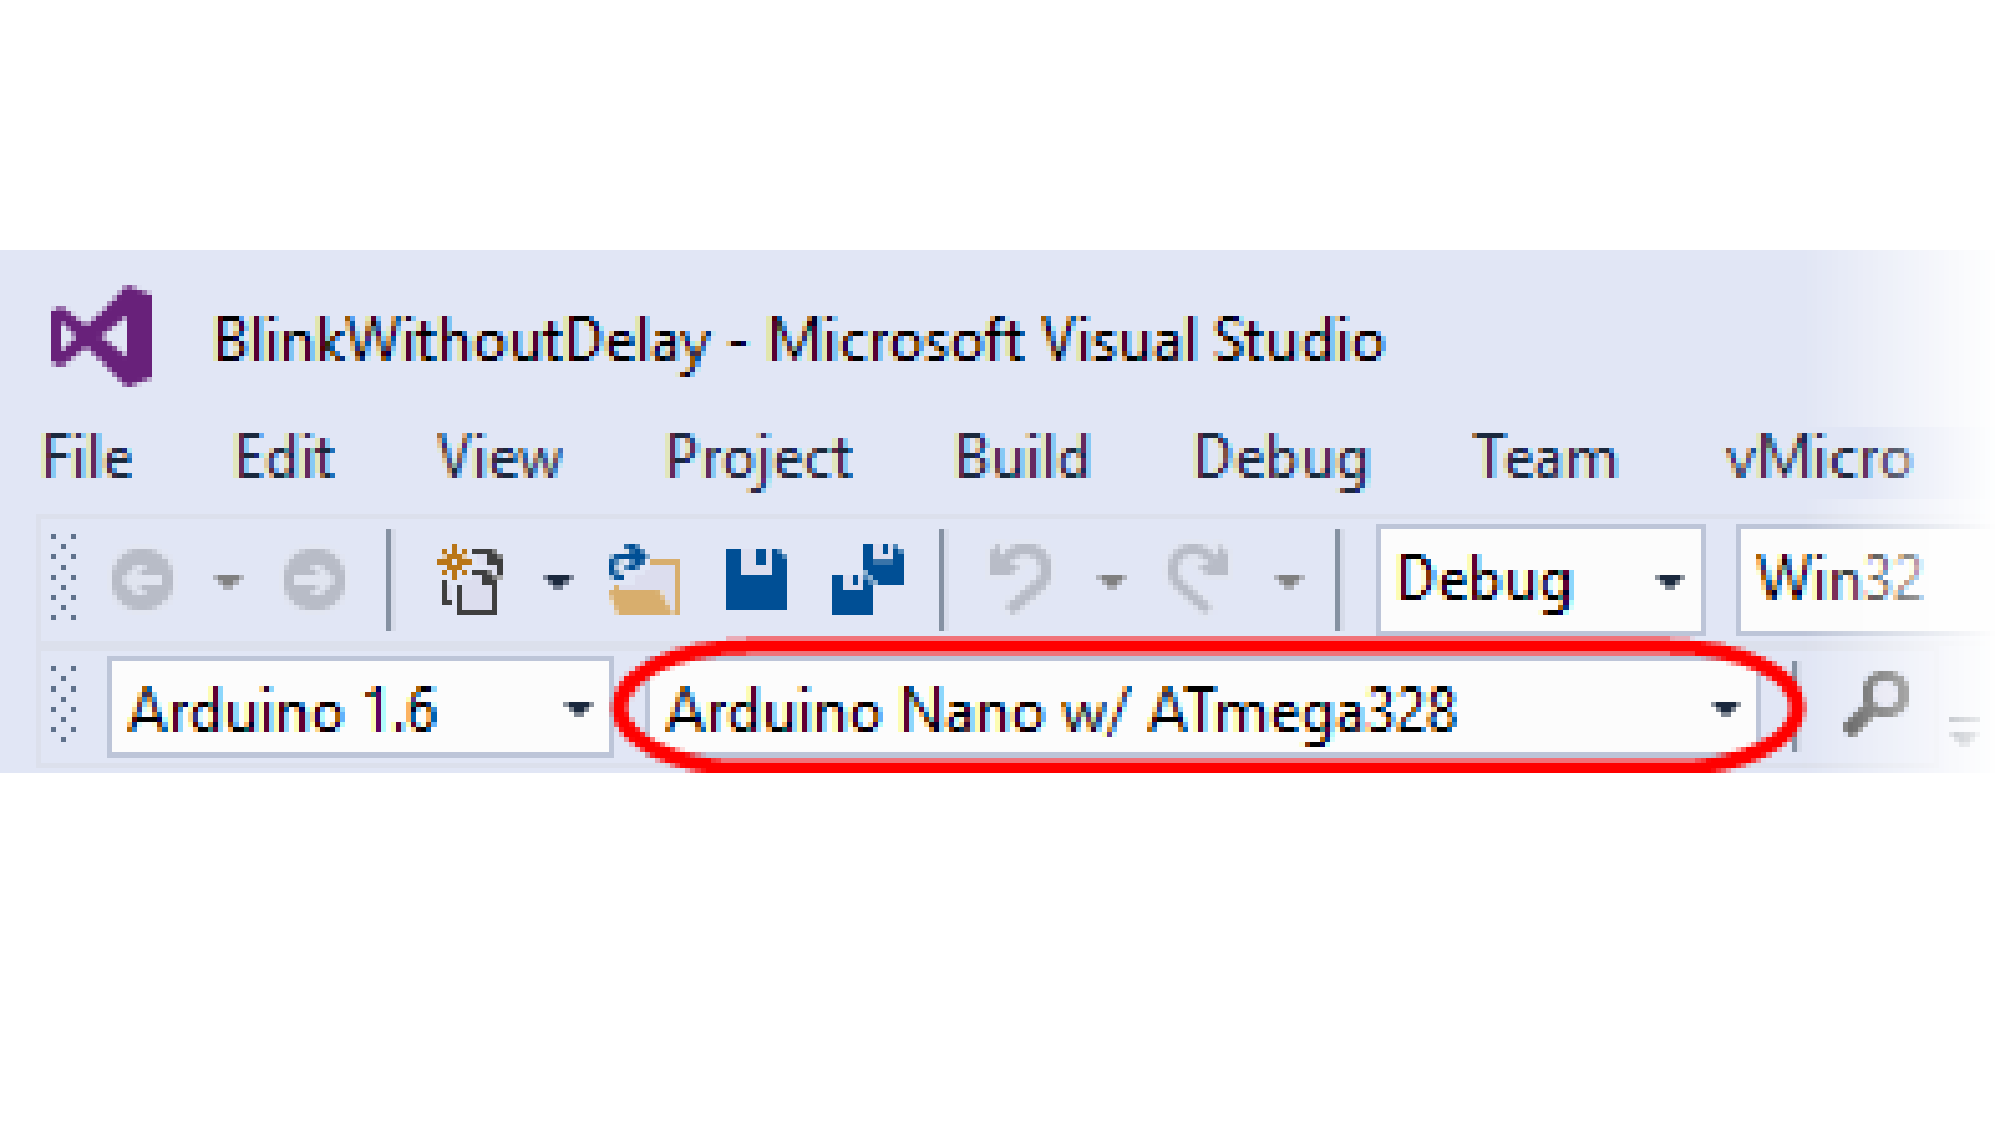
\includegraphics[width=0.7\linewidth]{./sdf/arduino_quantum_rx/figures/boardSelect.pdf}
	\caption{Selecting the Board Model.}
	\label{boardSelect}
\end{figure}

\subsubsection{Step 6}

Connect your Arduino board to your PC using a USB cable. You must also tell your IDE which serial port to use and for that purpose use the Visual Micro Serial Communications toolbar shown below in figure \ref{selectSerial}. If the Visual Micro Serial Communications toolbar is missing, then you can show it by right clicking in the toolbar area and checking "Micro Serial Communications".

\begin{figure}[H]
	\centering
	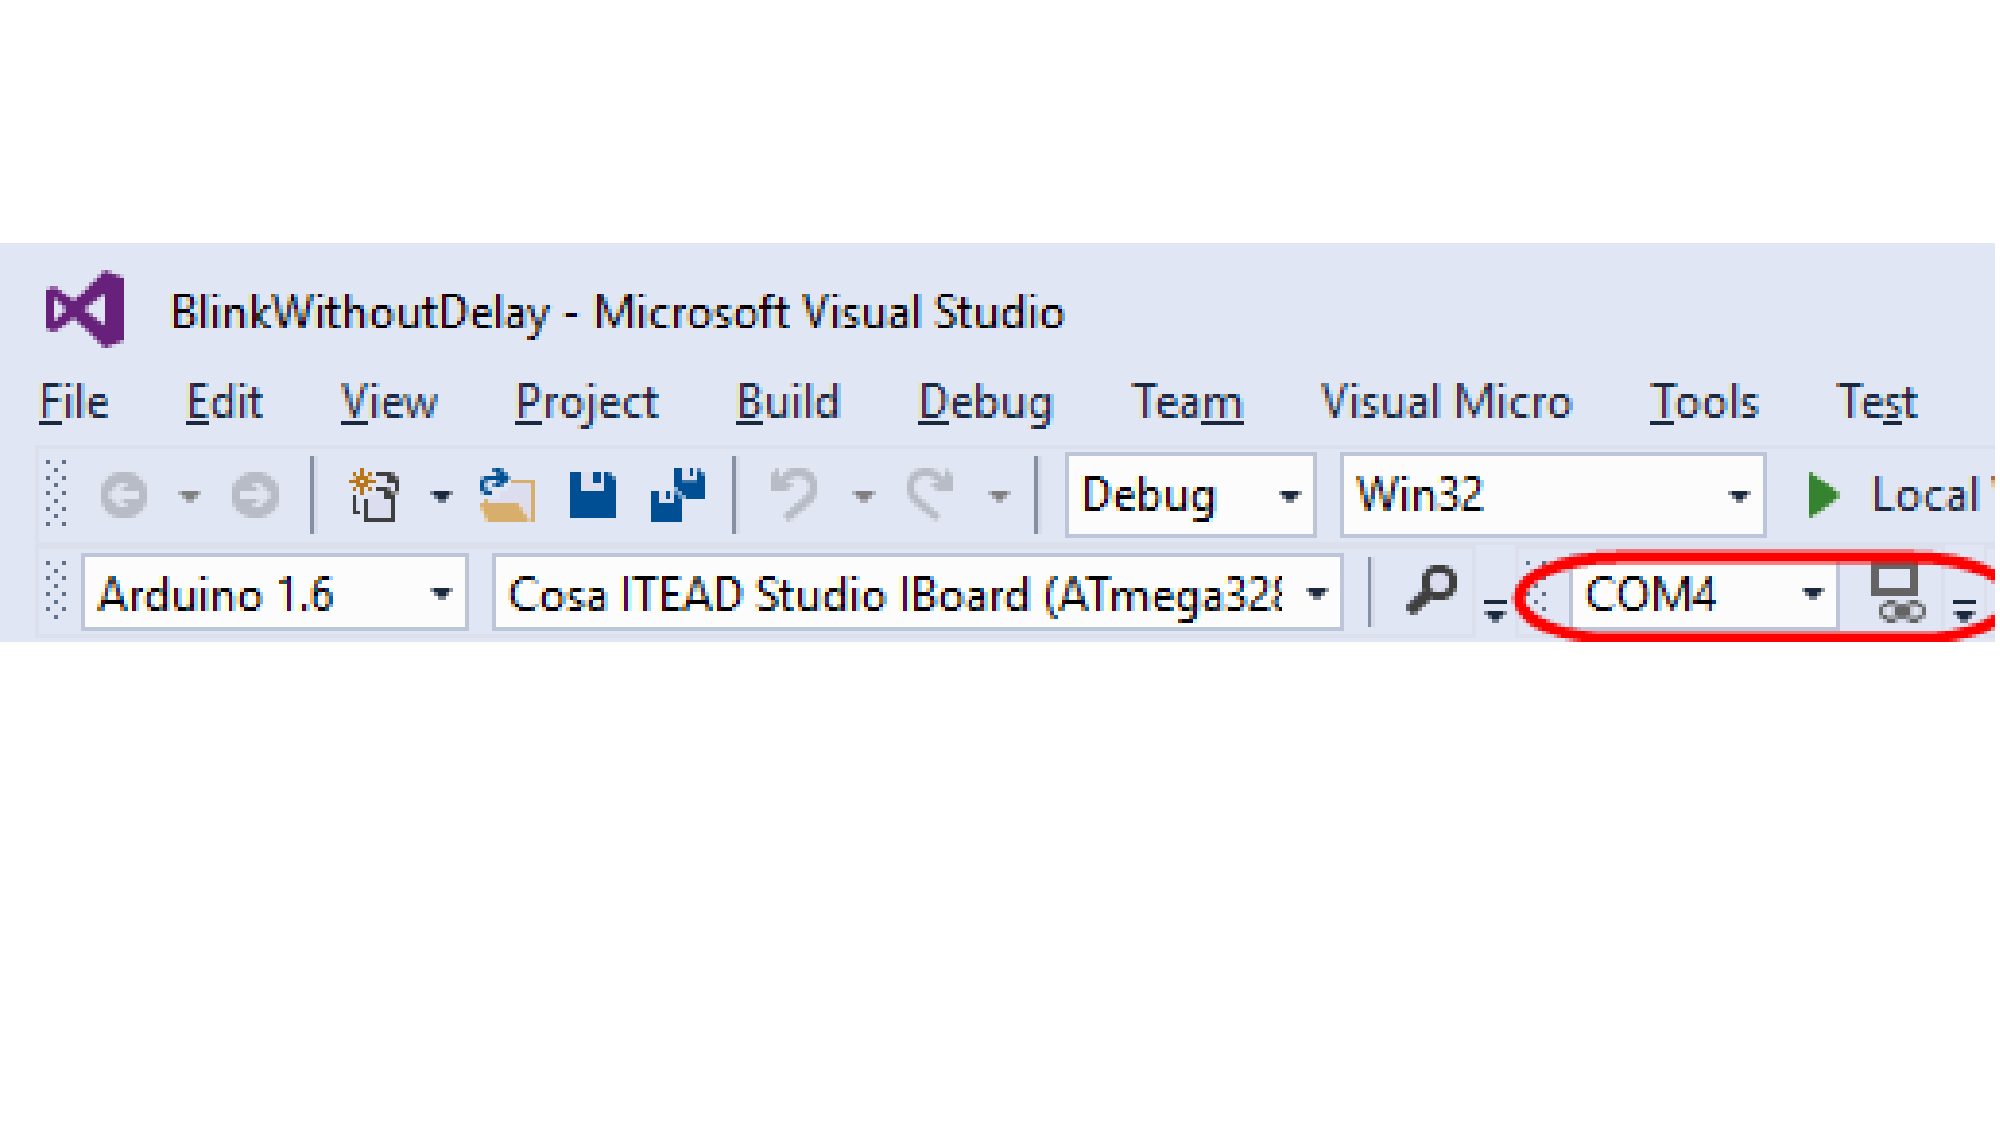
\includegraphics[width=0.7\linewidth]{./sdf/arduino_quantum_rx/figures/selectSerial.pdf}
	\caption{Setting up your Serial Port.}
	\label{selectSerial}
\end{figure}

\subsubsection{Step 7}
 At the end of these steps, you will be ready to write, compile, debug, and upload your Arduino sketches. In case of doubts consult the following link: https://www.visualmicro.com/page/User-Guide.aspx?doc=index.

% bibliographic references for the section ----------------------------
\clearpage
\printbibliography[heading=subbibliography]
\end{refsection}
\addcontentsline{toc}{subsection}{Bibliography}
\cleardoublepage
% ---------------------------------------------------------------------
